\documentclass[../TDM1-M2.tex]{subfiles}%

\begin{document}
\section[s]"1"{Masse attachée à 2 ressorts}

\enonce{%
	\noindent
	\begin{minipage}{0.75\linewidth}
		On considère un point M de masse $m$ attaché à deux ressorts identiques
		verticaux, de constante de raideur $k$ et de longueur à vide $\ell_0$. Les
		deux autres extrémités O et O' des ressorts sont fixes et espacées d'une
		distance $L$. On définit l'axe (O$z$) vertical ascendant.
	\end{minipage}
	\hfill
	\begin{minipage}{0.18\linewidth}
		\begin{center}
			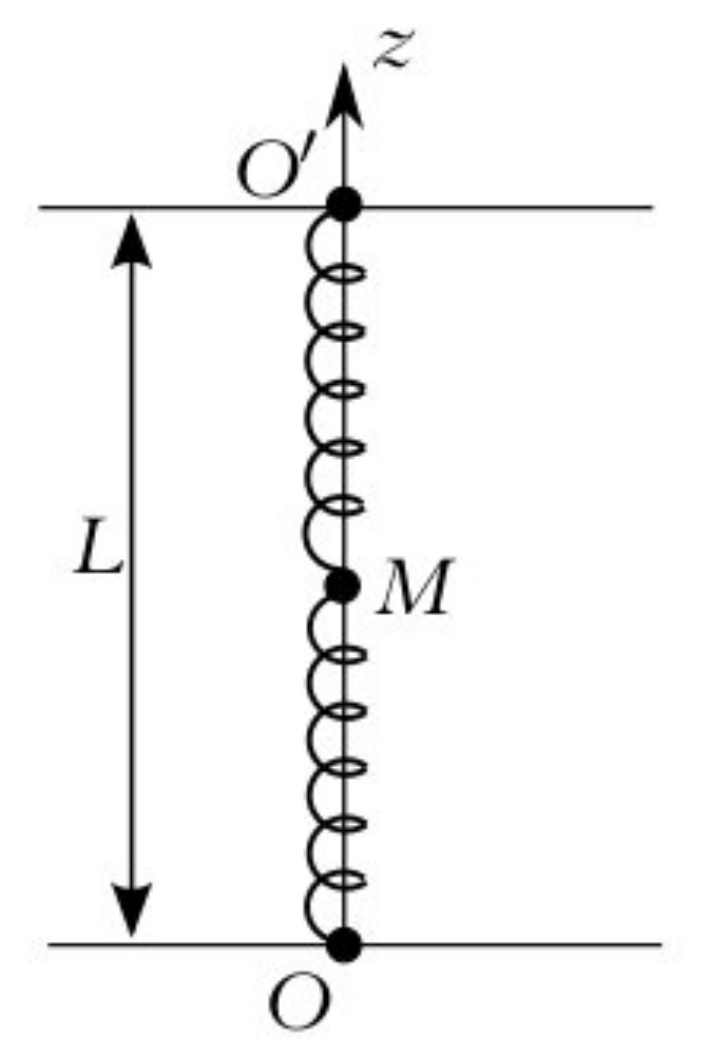
\includegraphics[width=\linewidth]{masse_2R-plain}
		\end{center}
	\end{minipage}
}

\QR{%
	Déterminer la position d'équilibre $z\ind{eq}$ de M.
}{%
	On étudie ici le point matériel M de masse $m$, dans le référentiel du
	laboratoire supposé galiléen avec le repère (O,$\uz$), $\uz$ vertical
	ascendant. On repère le point M par son altitude $\OMr = z(t)$.
	On effectue le \textbf{bilan des forces}~:
	\[
		\begin{array}{ll}
			\textbf{Poids}     & \Pf = m\gf = -mg\uz \\
			\textbf{Ressort 1} & \Ff\ind{ressort 1}
			= -k(\OMr - \ell_0)\uz = -k(z-\ell_0)\uz \\
			\textbf{Ressort 2} & \Ff\ind{ressort 2}
			= +k({\rm O'M} - \ell_0)\uz = +k(L-z-\ell_0)\uz
		\end{array}
	\]
	avec le ressort 1 celui d'en-dessous, le ressort 2 celui d'au-dessus. On
	notera simplement $\Ff_1$ et $\Ff_2$ dans la suite.
	Avec le PFD, on a
	\begin{gather*}
		m\af = \Pf + \Ff_1 + \Ff_2\\
		\Lra
		m\zpp = -mg -k(z - \cancel{\ell_0}) + k(L - z -\cancel{\ell_0})\\
		\Lra
		\boxed{\zpp + \frac{2k}{m}z = \frac{k}{m}L -g}
	\end{gather*}
	À l'équilibre, le ressort ne bouge plus~; on a donc $\zp = \zpp = 0$, et
	on trouve ainsi $z\ind{eq}$~:
	\[\boxed{z\ind{eq} = \frac{L}{2} - \frac{mg}{2k}}\]
	Sans la pesanteur, la masse sera à l'équilibre entre les deux ressorts,
	en toute logique. La gravité diminue cette altitude. On remarque que
	cette association de ressort est équivalente à avoir un seul ressort de
	raideur $2k$.
}

\QR{%
	Déterminer l'équation différentielle à laquelle satisfait $z(t)$.
	On écrira cette équation en fonction de $\w_0$ à définir et de
	$z\ind{eq}$.
}{%
	On a commencé la détermination de l'équation différentielle dans la
	question 2. On peut simplifier son expression en remarquant qu'à droite
	du signe égal, on doit trouver quelque chose homogène à $\w_0{}^2z$. On
	commence par identifier $\w_0$ avec la forme canonique~:
	\[\w_0 = \sqrt{\frac{2k}{m}}
		\qdonc
		\frac{k}{m}L - g = \w_0{}^2z\ind{eq}
	\]
	et finalement,
	\[\boxed{\zpp + \w_0{}^2z = \w_0{}^2z\ind{eq}}\]
}

\QR{%
	On écarte M d'une hauteur $a$ par rapport à sa position
	d'équilibre, et on le lâche sans vitesse. Déterminer $z(t)$.
}{%
	ion complète $z(t)$ et la somme de la solution particulière
	constante $z_p$ et de la solution homogène $z_h$. La solution
	particulière est, par définition, $z\ind{eq}$ (on l'a montré question 1).
	La solution homogène est celle d'un oscillateur harmonique, à savoir
	\[z_h = A\cos(\w_0t) + B\sin(\w_0t)\]
	Ainsi,
	\[z(t) = z\ind{eq} + A\cos(\w_0t) + B\sin(\w_0t)\]
	On trouve $A$ et $B$ avec les conditions initiales~:
	\begin{itemize}
		\item $z(0) = z\ind{eq} + a$ (masse lâchée d'une hauteur $a$ par
		      rapport à la position d'équilibre), or $z(0) = A + z\ind{eq}$,
		      donc
		      \[A = a\]
		\item $\zp(0) = 0$ (masse lâchée sans vitesse initiale), or $\zp(0)
			      = B\w_0$ donc
		      \[B = 0\]
	\end{itemize}
	\leftcenters{Ainsi,}{$\boxed{z(t) = z\ind{eq} + a\cos(\w_0t)}$}
}

\end{document}
